\documentclass[justified]{tufte-handout}
\usepackage{amsmath}
\usepackage{booktabs}
\usepackage{graphicx}
\graphicspath{{figures/}}

\title{Planar Camera Calibration with a Mobile Phone}
\author{Xu Xuanye, Student IDs: 24020036071 / H00490299}
\date{Robotics Integration Project I \quad 25 September 2026}

\begin{document}
\maketitle

\begin{abstract}
This experiment estimates a phone camera's intrinsic matrix and lens distortion
from 19 views of a planar checkerboard. All 19 images yielded the required
40 internal corners. OpenCV calibration returned an overall in-sample
reprojection RMS of 0.942 pixels at 4032 by 3024 resolution. The report
documents the actual inputs, fitted parameters, image evidence, and a
one-view sensitivity check. The board was displayed on a laptop screen;
its stated 25 mm square size was supplied for this experiment and was not
independently measured here.
\end{abstract}

\section{Aim and data}

The aim was to recover the intrinsic matrix \(K\) and distortion coefficients
of one phone camera using Zhang's planar calibration method
\citep{zhang1999}.\sidenote{The
phone model recorded in the converted image EXIF is Apple iPhone 14 Pro.
The individual lens is not identified by that field.}
Nineteen HEIC photographs were converted to JPEG with \texttt{heif-convert}
at quality 95. Every image is \(4032\times3024\) pixels. The pattern contains
9 by 6 squares, hence \(8\times5=40\) internal corners. The square length
entered in the program was \(s=0.025\) m. The checkerboard was shown on a
laptop display rather than printed. The Lab0 handout mentions a 3 cm
board; that dimension was not used for this screen pattern.

\section{Method}

For each accepted photograph, planar object points were defined as
\(M_{ij}=(is,js,0)^\mathsf{T}\). Image corners were detected with OpenCV
and refined to subpixel precision. The SB detector was available as a
fallback. With a different board pose in each view, the pinhole model is
\begin{equation}
  \lambda\widetilde{\boldsymbol m}
  =K[\,R\mid\boldsymbol t\,]\widetilde{\boldsymbol M},
  \qquad
  K=
  \begin{bmatrix}
  f_x&0&c_x\\
  0&f_y&c_y\\
  0&0&1
  \end{bmatrix}.
\end{equation}
OpenCV's \texttt{calibrateCamera} \citep{opencv_calibration} jointly fitted \(K\), the five reported
distortion coefficients, and a pose for each image. For \(N\) accepted
corners, the reported residual was independently recomputed as
\begin{equation}
 E_{\mathrm{RMS}}=
 \sqrt{\frac{1}{N}\sum_{i=1}^{N}
 \left\|\boldsymbol m_i-\widehat{\boldsymbol m}_i\right\|_2^2}.
\end{equation}
Here \(\widehat{\boldsymbol m}_i\) is the point returned by
\texttt{projectPoints}. This is an in-sample fit statistic, not a
measurement against an external reference.

\begin{figure*}[ht]
  \centering
  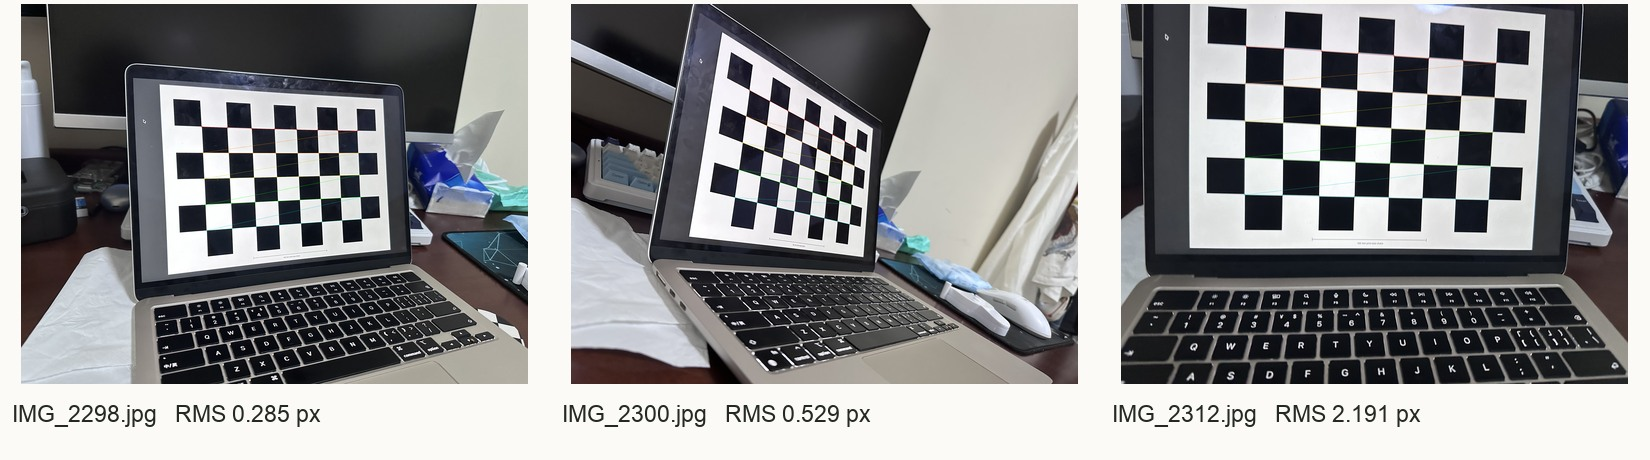
\includegraphics[width=\linewidth]{calibration_examples.jpg}
  \caption{Three accepted images with detected internal corners. The first
  two illustrate different viewing conditions; \texttt{IMG\_2312} has the
  largest per-image reprojection error. Figure labels give each view's RMS
  in pixels.}
\end{figure*}

\section{Results}

All \(19/19\) photographs were accepted. The fitted intrinsic matrix is
\begin{equation}
K=
\begin{bmatrix}
2859.815 & 0 & 2014.596\\
0 & 2856.387 & 1523.779\\
0 & 0 & 1
\end{bmatrix}\quad\text{pixels}.
\end{equation}
The coefficient vector in OpenCV order
\((k_1,k_2,p_1,p_2,k_3)\) is
\begin{equation}
(0.201096,\;-0.762019,\;-0.000094,\;0.000053,\;0.657344).
\end{equation}
The overall RMS is \(0.942\) px. The best individual view,
\texttt{IMG\_2298}, has \(0.285\) px RMS; \texttt{IMG\_2312}
has \(2.191\) px. The principal point is close to the image center
\((2016,1512)\), which is a useful plausibility check but not an
independent accuracy test.

\begin{figure*}[ht]
  \centering
  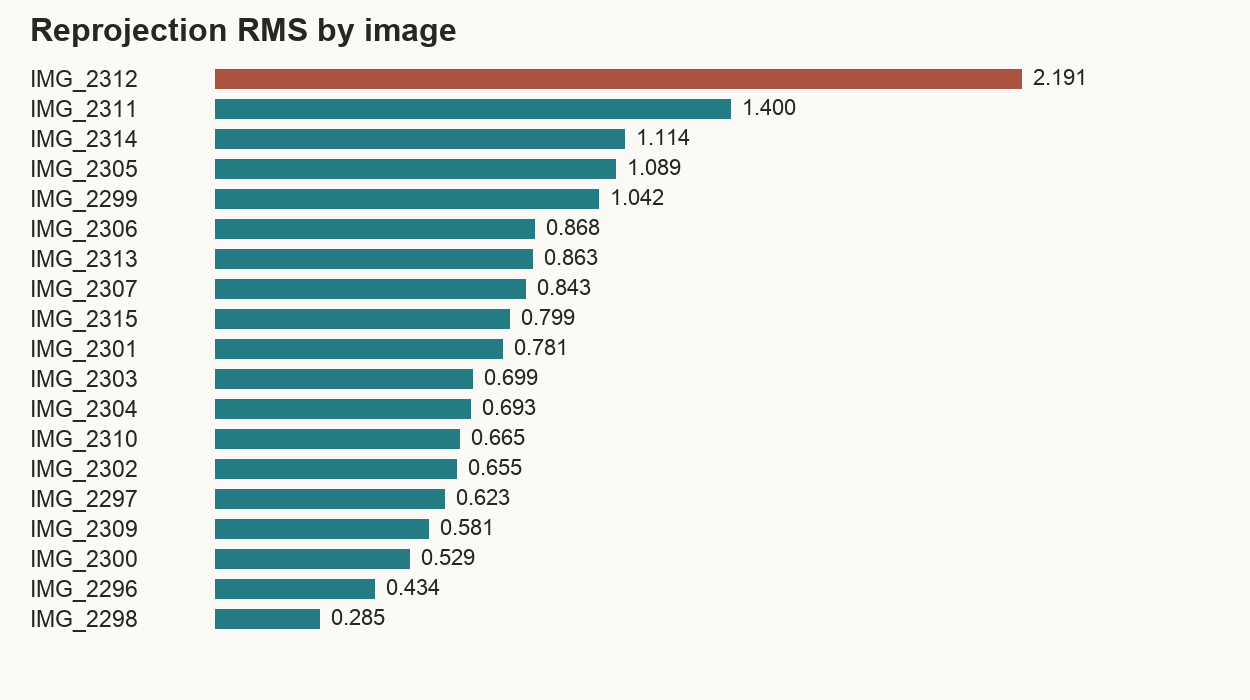
\includegraphics[width=\linewidth]{calibration_rms.png}
  \caption{Per-view reprojection RMS for all 19 photographs, sorted from
  largest to smallest. The highlighted view motivates the sensitivity
  check below.}
\end{figure*}

In a sensitivity check, \texttt{IMG\_2312} was omitted. Refitting
the other 18 photographs gave \(0.806\) px RMS, with
\(f_x\approx2854.3\) px and \(f_y\approx2852.1\) px.
The focal-length changes are below \(0.2\%\) relative to the 19-view
fit. The delivered parameters remain the 19-view result; this comparison
does not justify deleting an observation without checking its image.

\section{Interpretation and limits}

The images include changes in distance and orientation, which provide
constraints beyond a single frontal view. The relatively large higher-order
radial coefficients deserve caution: a screen pattern can introduce pixel
structure, glare, and interpolation effects, and only one dataset was
evaluated. No held-out calibration target or independent physical
measurement was used. Because the board's physical square length only
sets object-space scale, an error in the stated 25 mm size scales the
reported pose translations; it does not by itself change the pixel-valued
intrinsic matrix.

\section{Reproduction}

The run used Python 3.9.23, NumPy 2.0.2, and OpenCV 4.12.0.
From the repository root:
\begin{quote}\small\ttfamily
python3.9 lab0/code/calibrate\_phone.py\\
\quad --images lab0/data/phone\_jpg --square-size-m 0.025
\end{quote}
The complete per-image results, parameter array, and annotated images
are saved under \texttt{lab0/results/calibration/}. The report figures
were selected from those saved outputs.

\bibliographystyle{plainnat}
\bibliography{lab0_references}

\end{document}
